\documentclass[10pt,a4]{article}
\usepackage[english]{babel}
\usepackage[latin1]{inputenc}
\usepackage{subfigure}
\usepackage{epsfig}
\usepackage{amsmath}
\usepackage{amssymb}
\usepackage{color}
\parindent 0mm
\textwidth 16cm
\textheight 23cm
\oddsidemargin 0cm
\evensidemargin 0cm
\topmargin -10mm
\newcommand{\vect}[1]{{\bf{#1}}}
\newcommand{\svect}[1]{\boldsymbol{#1}}
\newcommand{\matr}[1]{\boldsymbol{#1}}


\begin{document}
\pagestyle{empty}
\begin{Large}
\begin{bf} 
T-61.5130 Machine Learning and Neural Networks\\ 
\end{bf}
\end{Large}
Karhunen, Hao Tele\\  
\\
\begin{large}
\begin{bf}
Exercise 1,  4.11.2011\\Model answer
\end{bf}
\end{large}

\begin{enumerate}

\item An odd sigmoid function is defined as
\begin{equation} \label{eq:sigmoid}
\varphi(v)=\frac{1-\exp(-av)}{1+\exp(-av)}=\tanh(av/2).
\end{equation}

The derivative:
\begin{equation}
\begin{split}
  \frac{d\varphi}{dv}&=\frac{a\exp(-av) (1 + \exp(-av)) + a\exp(-av)
    (1 - \exp(-av))} {(1+\exp(-av))^2} \\
  &= \frac{a ( \exp(-av) + \exp(-2av) + \exp(-av) - \exp(-2av) )}{(1 +
    \exp(-av))^2} \\
  &= \frac{a}{2} \frac{(1 + \exp(-av))^2 - (1 - \exp(-av))^2}{(1 +
    \exp(-av))^2} = \frac{a}{2} ( 1 - \varphi^2(v) )
\end{split}
\end{equation}

At the origin: 
\begin{equation}
\left.\frac{d\varphi}{dv}\right|_{v=0} = \frac{a}{2} (1 - \left(
  \frac{1 - \exp(-a * 0)}{1 + \exp(-a*0)} \right)^2 = \frac{a}{2}.
\end{equation}
\begin{equation}
  \mbox{When  $a$ $\rightarrow$ $\infty$,  $\varphi(v)$ $\rightarrow$} \left\{ 
    \begin{array}{rl}
      +1, &v > 0 \\
      -1, &v < 0 \\
      0, &v = 0
    \end{array} \right.
  \end{equation}

Fig.~\ref{fig:sigmoid} shows the values of the sigmoid
function~(\ref{eq:sigmoid}) with different values of $a$.

\begin{figure}[h]
  \begin{center}
    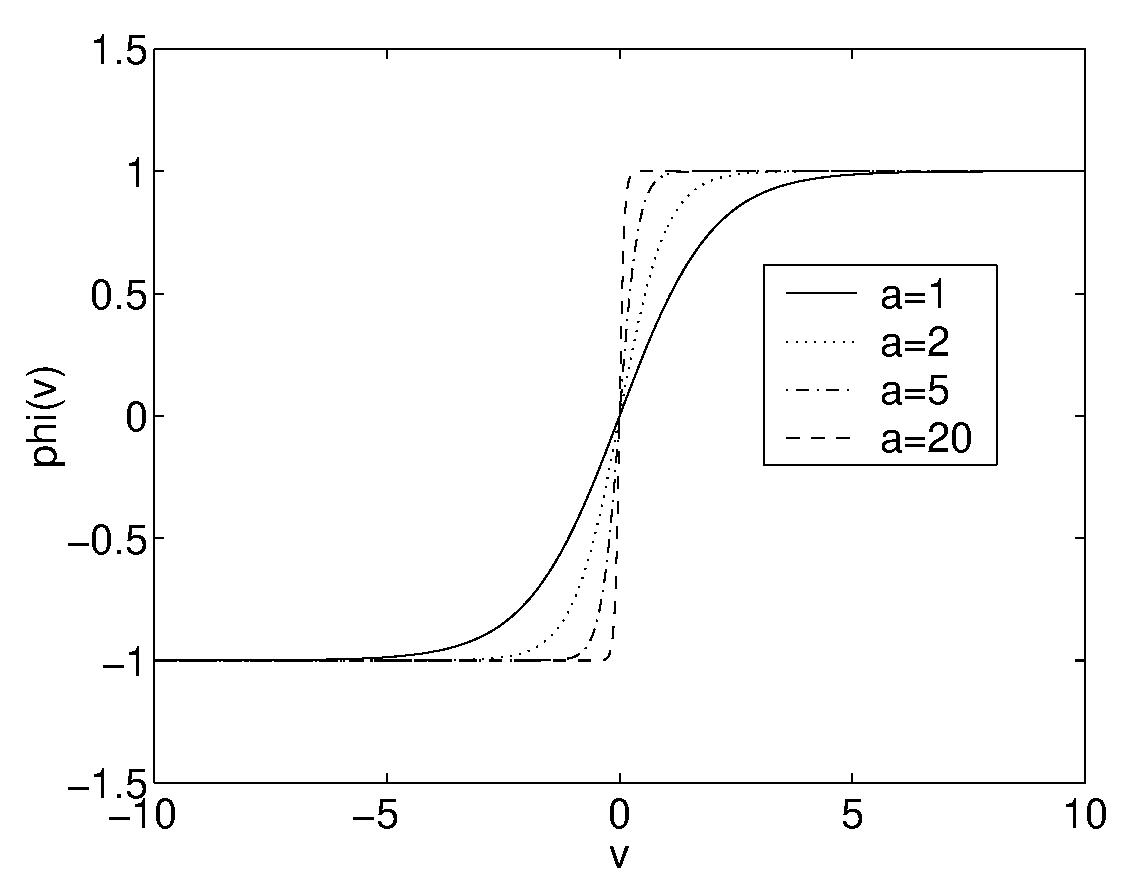
\includegraphics[width=12cm]{sigmoid.eps}
    \caption{\label{fig:sigmoid} Sigmoid function $\varphi(v)$ with
      different values of $a$. The function behaves linearly near the
      origin.}
  \end{center}
\end{figure}

\item 
  \begin{enumerate}
    
  \item The McCulloch-Pitts formula of a neuron is
    defined as a threshold function:
    \begin{equation}
      \varphi(v) = \left\{ \begin{array}{rl} 1, & v \geq 0 \\ 0, & v <
          0 \end{array} \right.,
    \end{equation}
    where $v_k = \sum_{j=1}^{m} w_{kj} x_j + b_k$, where $w_{kj}$'s are
    the synaptic weights and $b_k$ is the bias.
    
    A sigmoid activation function on interval $[0,1]$ is {\em e.g.}
    $\sigma(v) = 1 / (1 + \exp(-av))$, where we assume $a > 0$ without
    loss of generality.
    
    When synaptic weights have large values, also $|a v|$ tends to have
    a large value:
    \begin{equation}
      \begin{aligned}
        \lim_{a \rightarrow \infty} \sigma(v)& = \left. \frac{1}{1 +
            \exp(-av)}\right|_{a \rightarrow \infty} = \frac{1}{1+0} = 1 \mbox{\ \ \ \ \ \ ($v>0$)}
        \\
        \lim_{a \rightarrow \infty} \sigma(v)& = \left. \frac{1}{1 +
            \exp(-av)}\right|_{a \rightarrow \infty} =
        \frac{1}{1-\infty} = 0 \mbox{\ \ \ \ \ ($v<0$)}
      \end{aligned}
    \end{equation}
    
  \item We expand the $\exp(-av)$ in Taylor series around point $v=0$:
    
    \begin{equation}
      \begin{split}
      \sigma(v) &= \frac{1}{1 + \exp(-av)} = \frac{1}{1 + 1 - av +
        \underbrace{\frac{(av)^2}{2!} - \frac{(av)^3}{3!} +
          \cdots}_{\mbox{$\approx$ $0$, for small values of $v$}}} \\ 
      &\approx \frac{1}{2 ( 1 - \frac{av}{2})} \\
      &= \frac{1}{2} \frac{1 + \frac{av}{2}} {1 -
        \underbrace{\frac{(av)^2}{4}}_{\approx 0}} \approx \frac{1}{2}
      \left(1 + \frac{av}{2} \right) = L(v) \: _\Box
      \end{split}
    \end{equation}
    
  \end{enumerate}
  
\newpage
\item The fully recurrent network of 5 neurons.
 
  \begin{center}
    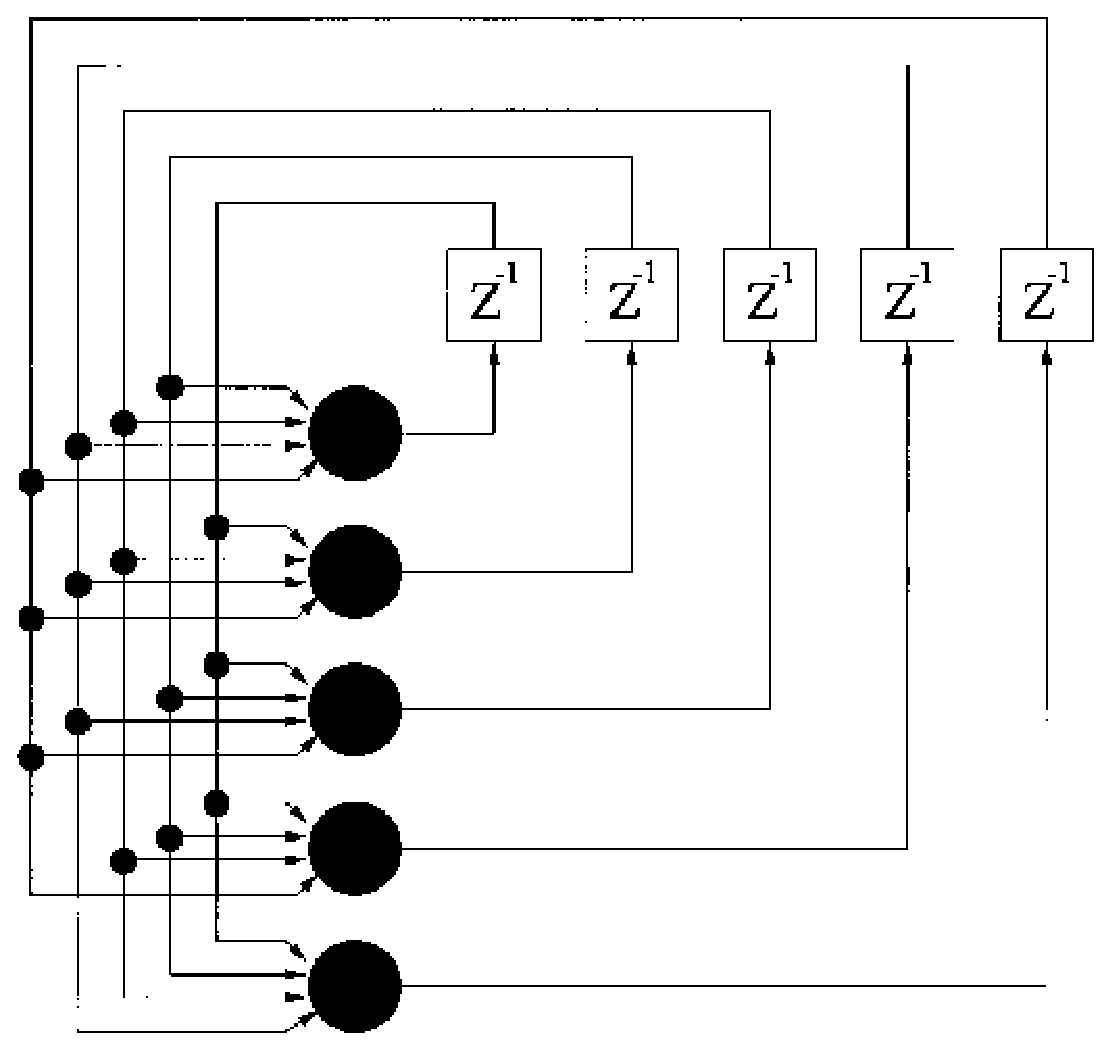
\includegraphics[width=12cm]{recurrent5.eps}
  \end{center}

  

\item A single neuron is depicted in Fig.~\ref{fig:singleneuron}


  \begin{figure}[hb]
    \begin{center}
      % use '../process_fig.sh neuron.fig' to make the .pstex_t
      \input neuron.pstex_t
      \caption{\label{fig:singleneuron} A single sigmoidal neuron.}
    \end{center}
  \end{figure}
  
  There the input $v_k$ to the nonlinearity $\varphi$ is defined as
  $v_k = \sum_{j = 0}^n w_{kj}x_j = \vect{w}_k^T \vect{x}$, \newline
  where $\vect{x}=\begin{pmatrix} 1 & x_1 &\cdots & x_n
  \end{pmatrix}^T$ and $\vect{w}_k=\begin{pmatrix} w_{k0} &\cdots &
    w_{kn} \end{pmatrix}^T$.

  When the neuron operates in its linear region, $\varphi(v) \approx
  \alpha v$ and $y_k \approx \alpha \vect{w}_k^T \vect{x}$. For the
  whole layer, this gives: 

  \begin{equation}
    \vect{y} = \begin{pmatrix}  y_1 \\ \cdots \\ y_m \end{pmatrix}
    \approx \alpha \begin{pmatrix}  \vect{w}_1^T \vect{x}\\ \cdots \\
      \vect{w}_m^T \vect{x} \end{pmatrix} 
    = \alpha \begin{pmatrix}  \vect{w}_1^T\\ \cdots \\
      \vect{w}_m^T \end{pmatrix} \vect{x} = \matr{W} \vect{x},
  \end{equation}
  where
  \begin{equation}
    \matr{W} = \alpha \begin{pmatrix}
      w_{10} & \cdots & w_{1n} \\ \vdots & \ddots & \vdots \\
      w_{m0} & \cdots & w_{mn} 
    \end{pmatrix}
  \end{equation}
  
  The whole network is constructed from these single layers:

  \begin{center}
    % use '../process_fig.sh network.fig' to make the .pstex_t
    \input network.pstex_t
  \end{center}
  
  and the output of the whole network is

  \begin{equation}
    \vect{y} = \matr{W_N} \vect{u_{N-1}} = \matr{W_N}  \matr{W_{N-1}}
    \vect{u_{N-2}} = \prod_{i = 1}^{N} \matr{W_i} \vect{x}.
  \end{equation}

  The product $\matr{T} = \prod_{i = 1}^{N} \matr{W_i}$ is a matrix of
  size $m \times n$: 

 \begin{equation}
    \vect{y} = \matr{T} \vect{x} = 
    \begin{pmatrix}
      t_{10} & \cdots & t_{1n} \\ \vdots & \ddots & \vdots \\
      t_{m0} & \cdots & t_{mn} 
    \end{pmatrix} \vect{x} = 
    \begin{pmatrix}  \vect{t}_1^T\\ \cdots \\
      \vect{t}_m^T 
    \end{pmatrix} \vect{x},
  \end{equation}
  
  which is exactly the output of a single layer linear network having
  $\matr{T}$ as the weights $_\Box$

\item 
\begin{enumerate} \item Fig.~\ref{fig:ex4a} shows the first
  signal-flow graph of a recurrent network made up of two neurons.

\begin{figure}[h] 
  \centering
      \input neuroEx1_4a.pstex_t
      \caption{The signal-flow graphs of the first recurrent network.}
  \label{fig:ex4a}
\end{figure}

From the figure it is evident that

\begin{equation}
  \left\{ \begin{aligned} u_1(n) & = x_2(n-1) \\  u_2(n) & = x_1(n-1)
    \end{aligned} \right. 
\end{equation}

On the other hand:
\begin{equation}
  \left\{ \begin{aligned} x_1(n) & = \varphi(w_1 u_1(n)) \\  x_2(n) & =
      \varphi (w_2 u_2(n))
    \end{aligned} \right. 
\end{equation}

By eliminating the $u_i$'s, we get
\begin{equation}
  \left\{ \begin{aligned} x_1(n) & = \varphi(w_1 x_2(n-1)) =
      \varphi(w_1 \varphi( w_2 x_1(n-2))) \\
      x_2(n) & = \varphi(w_2 x_1(n-1)) =
      \varphi(w_2 \varphi( w_1 x_2(n-2)))
    \end{aligned} \right. 
\end{equation}

These equations are 2nd order difference equations.

\item Fig.~\ref{fig:ex4b} shows the second signal-flow graph of a
  recurrent network made up of two neurons.

\begin{figure}[h] 
  \centering
      \input neuroEx1_4b.pstex_t
      \caption{The signal-flow graphs of the second recurrent network.}
  \label{fig:ex4b}
\end{figure}

Again from the figure:


\begin{equation}
  \left\{ \begin{aligned} 
      u_{11}(n) & = x_1(n-1) \\ 
      u_{21}(n) & = x_2(n-1) \\ 
      u_{12}(n) & = x_1(n-1) \\ 
      u_{22}(n) & = x_2(n-1) 
    \end{aligned} \right. 
\end{equation}
and
\begin{equation}
  \left\{ \begin{aligned} 
      x_1(n) & = \varphi(w_{11} u_{11}(n) + w_{21}u_{21}(n))\\  
      x_2(n) & = \varphi(w_{12} u_{12}(n) + w_{22}u_{22}(n))
    \end{aligned} \right. 
\end{equation}

Giving two coupled first order equations:
\begin{equation}
  \left\{ \begin{aligned} 
      x_1(n) & = \varphi(w_{11} x_{1}(n-1) + w_{21}x_{2}(n-1))\\  
      x_2(n) & = \varphi(w_{12} x_{1}(n-1) + w_{22}x_{2}(n-1))
    \end{aligned} \right. 
\end{equation}



\end{enumerate}
\end{enumerate}





\end{document}             % End of document.
